\documentclass[border=6pt]{standalone}
\usepackage{tikz}
\usetikzlibrary{arrows.meta,positioning,fit,backgrounds,calc}
\usepackage[T1]{fontenc}
\usepackage{lmodern}
\begin{document}
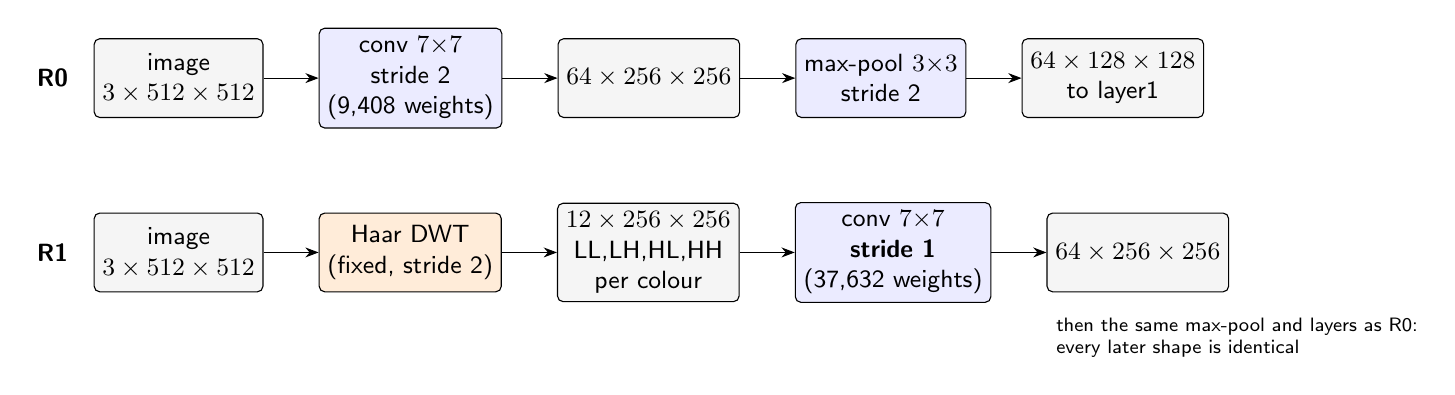
\begin{tikzpicture}[
  font=\sffamily\small, >=Stealth, node distance=5mm and 7mm,
  t/.style={draw, rounded corners=2pt, align=center, inner sep=3pt, fill=gray!8, minimum height=10mm},
  op/.style={draw, rounded corners=2pt, align=center, inner sep=3pt, fill=blue!8, minimum height=10mm},
  w/.style={draw, rounded corners=2pt, align=center, inner sep=3pt, fill=orange!15, minimum height=10mm},
  lab/.style={font=\sffamily\bfseries\small, anchor=east}]
% R0
\node[t] (x0) {image\\$3\times512\times512$};
\node[op, right=of x0] (c0) {conv $7{\times}7$\\stride 2\\(9{,}408 weights)};
\node[t, right=of c0] (f0) {$64\times256\times256$};
\node[op, right=of f0] (p0) {max-pool $3{\times}3$\\stride 2};
\node[t, right=of p0] (g0) {$64\times128\times128$\\to layer1};
\draw[->] (x0) -- (c0); \draw[->] (c0) -- (f0); \draw[->] (f0) -- (p0); \draw[->] (p0) -- (g0);
\node[lab] at ($(x0.west)+(-2mm,0)$) {R0};
% R1
\node[t, below=12mm of x0] (x1) {image\\$3\times512\times512$};
\node[w, right=of x1] (d1) {Haar DWT\\(fixed, stride 2)};
\node[t, right=of d1] (h1) {$12\times256\times256$\\LL,LH,HL,HH\\per colour};
\node[op, right=of h1] (c1) {conv $7{\times}7$\\\textbf{stride 1}\\(37{,}632 weights)};
\node[t, right=of c1] (f1) {$64\times256\times256$};
\draw[->] (x1) -- (d1); \draw[->] (d1) -- (h1); \draw[->] (h1) -- (c1); \draw[->] (c1) -- (f1);
\node[lab] at ($(x1.west)+(-2mm,0)$) {R1};
\node[font=\sffamily\scriptsize, align=left, anchor=north west] at ($(f1.south west)+(0,-2mm)$)
  {then the same max-pool and layers as R0:\\every later shape is identical};
\end{tikzpicture}
\end{document}
